%!TEX root = TIWSNE_Mini_project_main.tex
\section{Serial communication}

As stated in section \ref{sec:description}, the test data in this project written from a PC to the mote, and after completing the wireless transfer of image data, the data is transferred from the receiver mote to the PC for inspection and verification. This data transfer takes place using the USB serial connection of the telosb mote.

To ensure a reliable transfer, this project employs Automatic Repeat-reQuest(ARQ) of the Stop-and-Wait variant, which was explained in section \ref{sec:wireless} and shown on figure \ref{fig:ARQ}. This approach was chosen because it is the simplest, and because the bit error rate(BER) of the serial connection is negligible, rendering forward error correction(FEC) schemes irrelevant.

Because a PC is much faster than the mote - in particular the flash access on the mote - flow control was implemented for PC$\rightarrow$mote data transfers. A simplified sequence diagram is shown in figure \ref{fig:serialseq}.

\begin{figure}
\centering
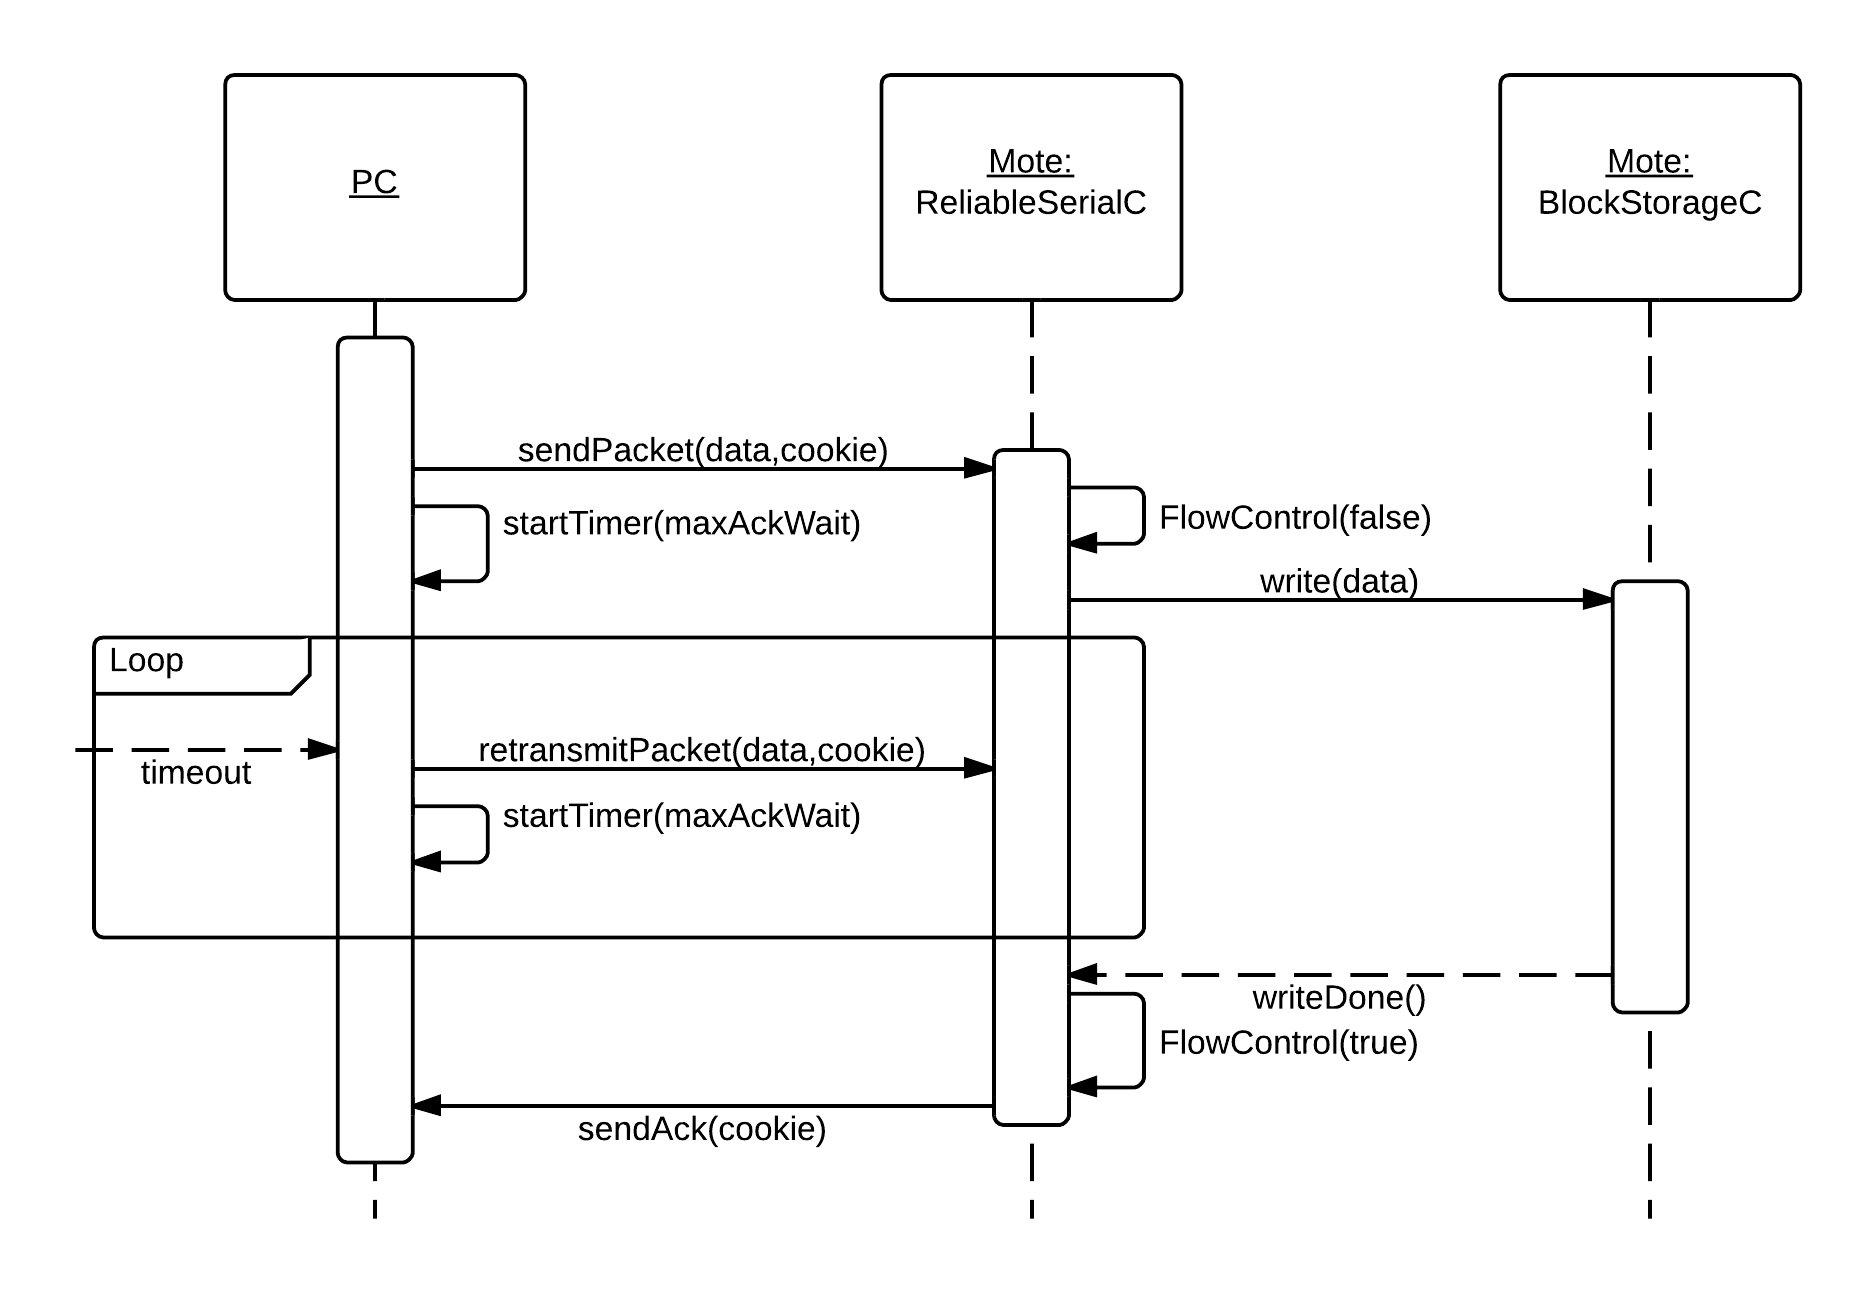
\includegraphics[width=0.8\linewidth]{serialseq}
\caption{Sequence diagram for PC$\rightarrow$mote transfer}
\label{fig:serialseq}
\end{figure}

The PC functionality was implemented in a java-program, which implements both sending and receiving from a mote. The PC program allows selecting which file to read/write to, thus enabling easier testing with different data.

%How image was made / reconstructed
%sequence diagram for pc-mote.
	%flow control
%mote-pc same as wireless sequence.
%ARQ vs FEC for serial connection.
%check ReliableSerialC
%how to use.